\section{Trenowanie}\label{sec:trenowanie}
\subsection{Sieć neuronowa}\label{subsec:siec_neuronowa}
\subsubsection{Architektura}\label{subsubsec:architektura}
Sieć neuronowa składa się z warstw wejściowych, ukrytych i wyjściowych. Można ją przedstawić jako graf skierowany acykliczny.
Wagi połączeń między neuronami są losowane na początku i aktualizowane w trakcie uczenia.
\begin{figure}[H]
    \centering
    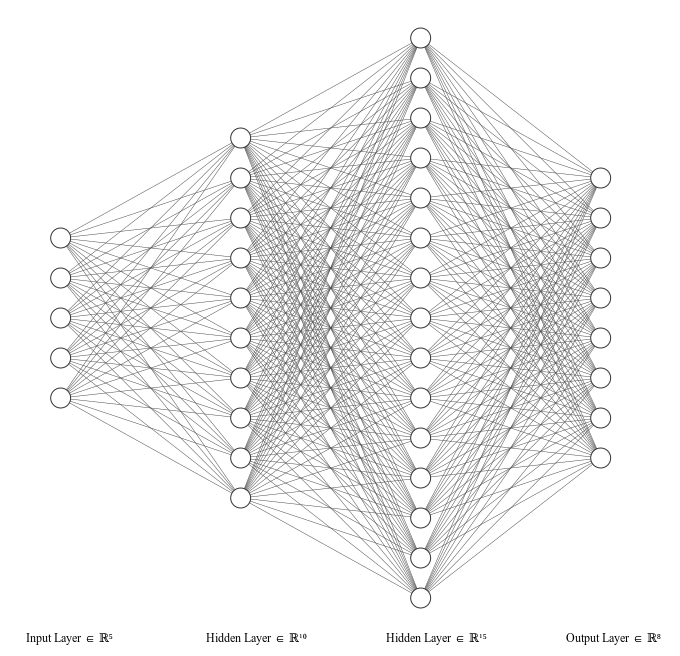
\includegraphics[width=0.6\textwidth]{img/nn.png}
    \caption{Poglądowy schemat sieci neuronowej.}
    \label{fig:neural_network}
\end{figure}
W tym badaniu ustalono optymalną architekturę sieci neuronowej na 4 warstwy:
\begin{itemize}
    \item warstwa wejściowa - 16 neuronów, po jednym na każdą cechę
    \item pierwsza warstwa ukryta - 128 neuronów
    \item druga warstwa ukryta - 256 neuronów
    \item warstwa wyjściowa - 26 neuronów, po jednym na każdą literę alfabetu angielskiego
\end{itemize}
\subsubsection{Funkcja aktywacji}\label{subsubsec:funkcja_aktywacji}
Funkcja aktywacji jest funkcją, która przekształca sumę ważoną wejść neuronu na jego wyjście.
Gdyby nie było funkcji aktywacji, to sieć neuronowa byłaby liniowa, a wtedy nie byłaby w stanie nauczyć się złożonych zależności.
W tym badaniu użyto funkcji ReLU na warstwach ukrytych (ang. \textit{Rectified Linear Unit}).
\begin{equation}
    \resizebox{0.3\textwidth}{!}{$f(x) = max(0, x)$}
\end{equation}
\begin{figure}[H]
    \centering
    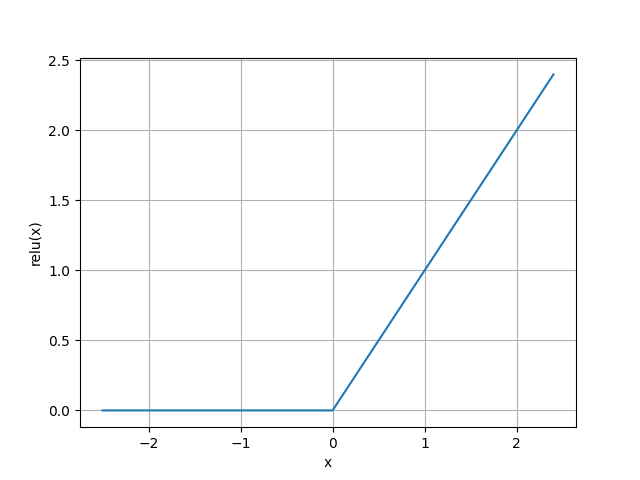
\includegraphics[width=0.6\textwidth]{img/relu.png}
    \caption{Funkcja ReLU.}
    \label{fig:relu}
\end{figure}
Na warstwie wyjściowej użyto funkcji softmax.
\begin{equation}
    \resizebox{0.3\textwidth}{!}{$f(x_i) = \frac{e^{x_i}}{\sum_{j=1}^{n} e^{x_j}}$}
\end{equation}
Opiera się ona na tym, że suma wszystkich wyjść jest równa 1. Dzięki temu można interpretować wyjścia jako prawdopodobieństwa.
Wybiera się neuron z największą wartością wyjścia, co daje wynik klasyfikacji.
\subsubsection{Funkcja straty}\label{subsubsec:funkcja_straty}
Funkcja straty jest funkcją, która określa jak bardzo wynik klasyfikacji różni się od oczekiwanego.
Ze względu na to, że wyjście sieci neuronowe nie jest jako wektor one-hot
(wektor, w którym tylko jedna wartość jest równa 1, a reszta 0),
wykorzystano funkcję entropii krzyżowej kategorycznej (ang. \textit{sparse categorical cross-entropy}).
\begin{equation}
    \resizebox{0.3\textwidth}{!}{$f(y, \hat{y}) = -\sum_{i=1}^{n} y_i \log(\hat{y_i})$}
\end{equation}
Gdzie $y$ to wektor oczekiwanych wyjść, a $\hat{y}$ to wektor wyjść sieci neuronowej.
\subsubsection{Uczenie sieci}\label{subsubsec:uczenie_sieci}
Uczenie sieci neuronowej polega na aktualizacji wag połączeń między neuronami.
Najważniejszymi parametrami podczas trenowania sieci neuronowej są:
\begin{itemize}
    \item współczynnik uczenia (ang. \textit{learning rate}). Określa jak bardzo aktualizowane są wagi po każdej iteracji.
    \item funkcja optymalizująca (ang. \textit{optimizer}). Określa jak aktualizowane są wagi po każdej iteracji.
    \item funkcja straty (ang. \textit{loss function}). Określa jak bardzo wynik klasyfikacji różni się od oczekiwanego.
    \item liczba epok (ang. \textit{epochs}). Określa ile razy sieć neuronowa przejdzie przez cały zbiór danych.
\end{itemize}
W tym badaniu użyto następujących parametrów:
\begin{itemize}
    \item współczynnik uczenia - 0.001
    \item funkcja optymalizująca - Adam
    \item funkcja straty - entropia krzyżowa kategoryczna
    \item liczba epok - 40
\end{itemize}
\subsection{K najbliższych sąsiadów}\label{sec:k_najblizszych_sasiadow}